\documentclass{article}

\author{Asaf Badouh, Alexander Parunov}
\title{AMMM Course Project Report\\ \textbf{Nurses in Hospital}}
\date{\today}

\usepackage{graphicx}
\usepackage{amsmath}
\usepackage{amssymb}
\usepackage{listing}
\usepackage{algpseudocode}

\graphicspath{ {images/} }
\newcommand\tab[1][1cm]{\hspace*{#1}}

\begin{document}
	\maketitle
	\pagebreak
	
	\section{Problem Statement}
\tab A public hospital needs to design the working schedule of their nurses. We know for, for each hour \textit{h}, that at least $demand_h$ nurses should be working. We have available a set of \textit{nNurses} and we need to determine at which hours each nurse should be working. However following constraints must be met:
	\begin{enumerate}
		\item Each nurse should work at least \textit{minHours} hours.
		\item Each nurse should work at most \textit{maxHours} hours.
		\item Each nurse should work at most \textit{maxConsec} consecutive hours.
		\item No nurse can stay at the hospital for more than \textit{maxPresence} hours (e.g. is \textit{maxPresence} is 7, it is OK that a nurse works at 2am and also at 8am, but it not possible that he/she works at 2am and also at 9am).
		\item No nurse can rest for more than one consecutive hour (e.g. working at 8am, resting at 9am and 10am, and working again at 11am is not allowed, since there are two consecutive resting hours).
	\end{enumerate}
\tab The goal is to determine at which hours each nurse should be working in order to \textbf{minimize} the \textbf{number of nurses} required and satify all above given constrains.
	\section{Integer Linear Model}
\tab Before defining the model and formal solution, set of parameters and decision variables that are used in model must be defined.
	\subsection{Parameters}
	\begin{itemize}
		\item \textit{nNurses:} Int - number of nurses
		\item \textit{nHours:} Int - number of hours
		\item \textit{minHours:} Int - minimum hours each nurse should work
		\item \textit{maxHours:} Int - maximum hours each nurse can work
		\item \textit{maxConsec:} Int - maximum consecutive hours each nurse can work
		\item \textit{maxPresence:} Int - maximum number of hours each nurse can be present
		\item $demand_h[nNurses]:$ Int - demanded number of working nurses at each hour, indexed $h$
	\end{itemize}
	
	\subsection{Decision Variables}
	\begin{itemize}
		\item $works_{n,h}[nNurses][nHours]:$ Boolean - Nurse $n$ works at hour $h$
		\item $WA_{n,h}[nNurses][nHours]:$ Boolean - Nurse $n$ works after hour $h$
		\item $WB_{n,h}[nNurses][nHours]:$ Boolean - Nurse $n$ worked before hour $h$
		\item $Rest_{n,h}[nNurses][nHours]:$ Boolean - Nurse $n$ rests at hour $h$. However, nurse should have worked before and should work after the resting hour $h$. Otherwise it's not considered as resting hour.
		\item $used_n[nNurses]:$ Boolean - Nurse $n$ is working
	\end{itemize}
	
	\subsection{Objective Function}
\tab After defining all parameters and decision variable we might proceed with definition of objective function and formal constaints. In addition to that,for clarity, we denote set of \textit{nHours} as $H$, and set of \textit{nNurses} as $N$. So, since the goal of project is to have as few working nurses as possible satisfying $demand_n[nNurses]$ and all constraints, the objective function is:
\begin{equation}
	\min \sum_{n=1}^N used_n 
\end{equation}
	\subsection{Constraints}
\tab Solution of problem must respect all constraints given in Section 1. Moreover, ILOG model direcly resembles formally stated constraints. Which means, after formally defining constraints, we may obtain an Integer Linear solution. So constraints are following:\\\\

\tab \textbf{Constraint 1:} On each hour $h$ at least $demand_h$ nurses should work.\\
\begin{minipage}{\linewidth}
	\begin{equation}
		\sum_{n=1}^N works_{n,h} \geq demand_h, \forall h \in H
	\end{equation}
\end{minipage}

\tab \textbf{Constraint 2:} Each nurse $n$ should work at least $minHours$ minimum number of hours.\\
\begin{minipage}{\linewidth}
	\begin{equation}
		\sum_{h=1}^H works_{n,h} \geq used_n \times minHours, \forall n \in N
	\end{equation}
\end{minipage}

\tab \textbf{Constraint 3:} Each nurse $n$ can work at most $maxHours$ maximum number of hours.\\
\begin{minipage}{\linewidth}
	\begin{equation}
		\sum_{h=1}^H works_{n,h} \leq used_n \times minHours, \forall n \in N
	\end{equation}
\end{minipage}

\tab \textbf{Constraint 4:} Each nurse $n$ can work at most $maxConsec$ maximum consecutive hours.\\
\begin{minipage}{\linewidth}
	\begin{equation}
		\sum_{j=i}^{i+maxConsec} works_{n,j} \leq used_n \times maxConsec, \forall n \in N, \forall i \in [1,nHours-maxCosec]
	\end{equation}
\end{minipage}

\tab \textbf{Constraint 5:} No nurse $n$ can stay at the hospital for more than $maxPresence$ maximum present hours. In other words, if the nurse worked at hour h, he/she cannot work after $h+maxPresence$ hour.\\
\begin{minipage}{\linewidth}
	\begin{equation}
		WB_{n,h} + WA_{n,h+maxPresence} \leq 1, \forall n \in N, \forall h \in \{h \in H|h \leq nHours-maxPresence \}
	\end{equation}
\end{minipage}

\tab \textbf{Constraint 6:} No nurse $n$ can rest for more than one consecutive hour.\\
\begin{minipage}{\linewidth}
	\medskip $\forall n \in N, \forall h \in \{h \in H|h \leq nHours-1 \}$
	\begin{equation}
		WA_{n,h} \geq WA_{n,h+1}
	\end{equation}
	\begin{equation}
		WB_{n,h} \leq WB_{n,h+1}
	\end{equation}
	\begin{equation}
		Rest_{n,h} + Rest_{n,h+1} \leq 1
	\end{equation}
\end{minipage}
\\\\
\tab In order to connect $WB_{n,h}, WA_{n,h}$ and $Rest_{n,h}$ decision variable matrices with a solution matrix $works_{n,h}$, we need to construct following logical equivalence:\\
\begin{minipage}{\linewidth}
	\begin{equation}
		Rest_{n,h} == (1-works_{n,h}) - (1-WA_{n,h}) - (1-WB_{n,h})
	\end{equation}
\end{minipage}
\\\\
\tab Which means:\\\\
If $Rest_{n,h} = 1$, then $(1-works_{n,h}) - (1-WA_{n,h}) - (1-WB_{n,h}) = (1-0) - (1-1) - (1-1) = 1$.\\\\
If $Rest_{n,h} = 0$, then $(1-works_{n,h}) - (1-WA_{n,h}) - (1-WB_{n,h}) = (1-0) - (1-1) - (1-0) = 0$\\\\

If feasible solution exists, then we get filled matrix $works_{n,h}$ and array of used nurses $used_n$ with minimized value of objective function $\min \sum_{n=1}^N used_n$. Which means this optimization problem is solved.
	\section{Metaheuristics}
\tab Integer Linear program guarantees to find an optimal solution if any feasible solution exists. However, this can be quite time consuming for medium and big size problems. That's why it's necessary to introduce some heuristics and solve this combinatorial optimization problem using them. Which assumingly should give a worse solution than OPL, but faster. We will consider two meta-heuristics: \textbf{GRASP} and \textbf{BRKGA}.
	\subsection{GRASP}
\tab The essence of GRASP is to select a candidate for solution element from a set of candidate elements using some criteria, which will be discussed later. First of all we need to generate that candidate set. The working nurse might be viewed as a boolean array, where \textit{1} means nurse works on that hour, and \textit{0} means nurse doesn't work. An example nurse boolean array might look like that: [0, 1, 1, 1, 1, 0, 0, 0]. And this working nurse is exactly the candidate element for solution. In order to increase time efficiency and solution accuracy, we generate all possible elements for hours $h \in [1,19]$ and save it locally. Then before starting solving problem, we filter that set of candidate elements so that it corresponds to specific constraints, given by parameters. Even if the set doesn't exist it still takes around 8 secs to generate all $2^{19} - 1 = 524287$ possible elements for hour $h = 19.$ And after initial generation, we can load elements from computer. This will improve speed of program. However, in case $h \geq 20$, generating all possible candidate elements and storing them locally is highly time and space consuming. So instead, we temporarily generate randomly $4 \times nNurses$ feasible candidate elements, respecting all given constraints. And then use this set to solve our problem. In case of $nNurses = 1800$, it takes around 8 secs to generate this set of feasible element solutions. Our \textbf{GRASP} just like any other is divided into two phases \textit{Constructive Phase} and \textit{Local Search Phase}, with modifications of phases themselves.
	\subsubsection{Constructive Phase}
		\begin{algorithmic}[1]
		\Function{construct}{gc(.),$\alpha$}
			\State Initialize candidate set C;
			\State $\underline{s} = min\{g(t) | t \in C \}$
			\State $\overline{s} = max\{g(t) | t \in C \}$
			\State $RCL = \{s \in C | gc(s) \leq \underline{s} + \alpha(\overline{s} - \underline{s}) \}$
			\State Select candidate element $x$, at random, from $RCL$
			\State \Return x 
		\EndFunction
		\end{algorithmic}
\tab So instead of classical \textbf{GRASP} \textit{Constructive Phase}, where candiate solution is constructed, we return one candidate element for overall solution. In most of the cases random candidate element is not the best, so we perform a \textit{Local Search} on returned candidate element $x.$\pagebreak
	\subsubsection{Local Search Phase}
	\begin{algorithmic}[1]
	\Function{localSearch}{x, C, $\alpha$, $nHours$}
		\State $maxDistance = \sqrt{nHours} \times (1-\alpha)$
		\State $N(x) = \{t \in C | dist(x,t) \leq maxDistance \}$
		\ForAll{$n \in N$}
			\If{$gc(n) < gc(x)$}
				\State x = n
			\EndIf
		\EndFor
		\State \Return x
	\EndFunction
	\end{algorithmic}
\tab LOCALSEARCH function will return the best element in a neighborhood of candidate element, where neighborhood is defined by Euclidean distance from that element. The radius of neighborhood is also determined by $\alpha$ parameter. In case $\alpha = 0$, we get the greediest approach, which is the best and slowest at the same time.\\
\tab The difference between classical \textbf{GRASP} and \textbf{ours}, is that we don't construct the set of candidate solutions, and then perform \textit{Local Search} on that set. But rather randomly return 1 element from constructed $RCL$ and apply local search on 1 element. This will reduce execution time, while returning same locally optimal candidate element. To conclude \textbf{GRASP} let's introduce our \textit{Greedy Cost function}
	\subsubsection{Greedy Cost Function}
	\begin{algorithmic}[1]
	\Function{greedyCost}{x, demand}
		\State Calculate positive hits: $posHits$
		\State Calculate negative hits: $negHits$
		\State $demand = demand-x$
		\State $hitsDiff = posHits - negHits$
		\State $cost = e^{-hitsDiff}$
		\State \Return $(demand, cost)$
	\EndFunction
	\end{algorithmic}
\tab Above given \textit{Greedy Cost function} will return updated demand and cost of candidate element. In order to understand this \textit{function} let's consider following example:
	\begin{itemize}
		\item $demand = [1,2,3,-2,4,-5,-6]$
		\item $x = [1,0,0,1,1,0,0]$
	\end{itemize}
\tab \textit{Positive Hits} is number of times $x$ decreases from positive values of $demand$, while \textit{Negative Hits} is number of times $x$ decreases from negative values of $demand.$ So in above given example, $posHits = 2$ and $negHits = 1.$ Since our goal is preferebly to decrease positive values of leftover demand, $hitsDiff$ is used. After that, exponential function is applied to $hitsDiff$, because we want to exponentially decrease/increase cost in case of wrong/right candidate element and choose the maximum cost. Since we have minimization problem, we invert exponential function, i.e. $\max e^{hitsDiff} = \min e^{-hitsDiff}$. 
	\subsection{BRKGA}
	\section{Comparative Results}
\tab Before starting comparing results of metaheuristics and ILP, let's find the most optimal alpha parameter. This should be done on following pretty big instance size, to see tentative difference:
\begin{itemize}
	\item \small \textit{nNurses=1800}
	\item \small \textit{nHours=24}
	\item \small \textit{minHours=6}
	\item \small \textit{maxHours=18}
	\item \small \textit{maxConsec=7}
	\item \small \textit{maxPresence=24}
	\item \small \textit{demand=[964, 650, 966, 1021, 824, 387, 828, 952, 611, 468, 403, 561, 862, 597, 1098, 855, 918, 1016, 897, 356, 615, 670, 826, 349]}
\end{itemize}

\begin{figure}[!htbp]
	\caption{GRASP: Alpha vs Time \& Objective Function Value}
	\center{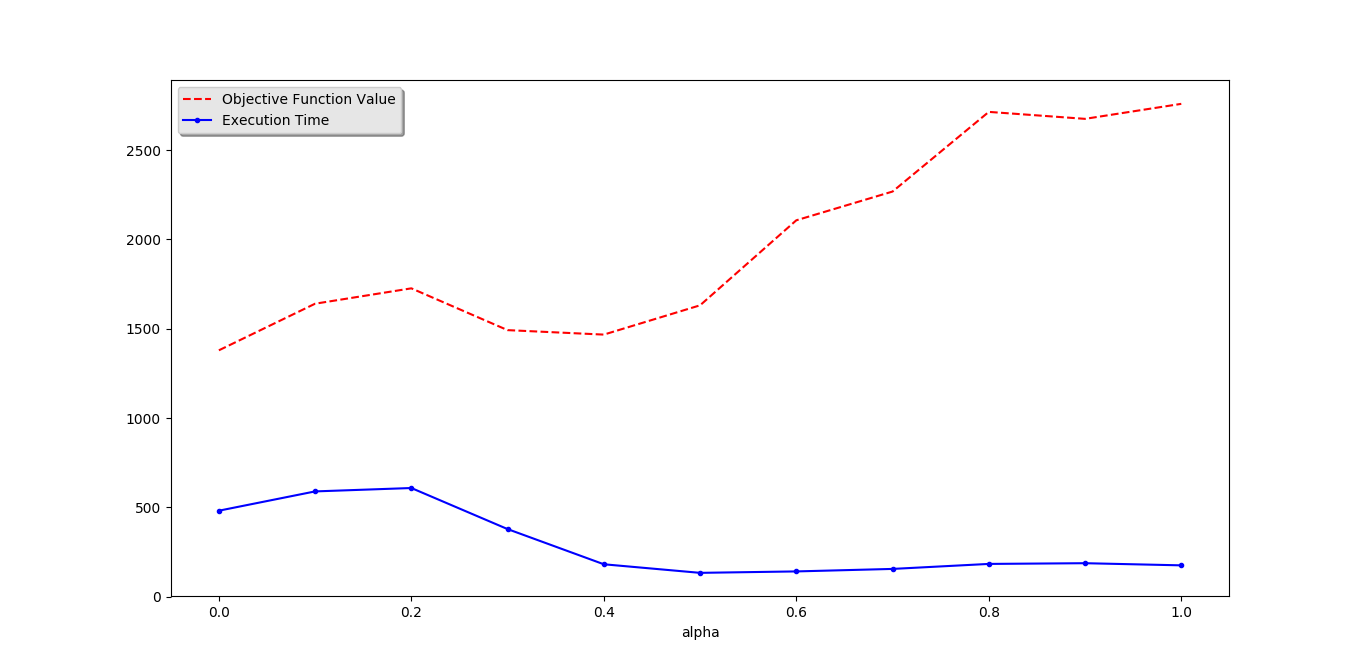
\includegraphics[scale=0.35]{grasp_vs_alpha.png}}
	\label{fig:graspalpha}
\end{figure}
\tab From Figure~\ref{fig:graspalpha} we can clearly see that the most optimal value of $\alpha$ parameter is $0.4$ both timewise and objective function valuewise. Which means, we will use this $\alpha$ parameter for all future executions. 
\end{document}